\section{Dipendenza della frequenza dalla massa lineare}

In quest'ultima sezione è stata analizzata la proporzionalità inversa della frequenza di risonanza dalla radice quadrata della massa lineare della corda.  
Sono state utilizzate quattro corde differenti, mantenendo costante la tensione e fissando la lunghezza del tratto vibrante: anche in questo caso si è studiata la seconda armonica.
I valori misurati di massa e lunghezza sono: $m = \qty{280.4 \pm 0.5}{g}$ e $L = \qty{0.697 \pm 0.015}{m}$. 
Le misure sono riportate nella Tabella 4.

\begin{table}[H]
\centering
\begin{tabular}{cccc}
\hline
Corda & $\mu$ (kg/m) & $f_2$ (Hz) & $\sigma_{f_2}$ (Hz) \\
\hline
Verde fluo & 0.002281 & 52.0 & 0.5 \\
Gialla e nera & 0.002368 & 51.0 & 0.5 \\
Nera & 0.002020 & 55.0 & 0.5 \\
Rossa & 0.002099 & 54.0 & 0.5 \\
\hline
\end{tabular}
\caption{Masse lineari, frequenze e incertezze.}
\end{table}

Avvalendosi di \eqref{eq:frequenze}, si interpolano linearmente i dati come mostrato in Figura 4.

\begin{figure}[H]
    \centering
    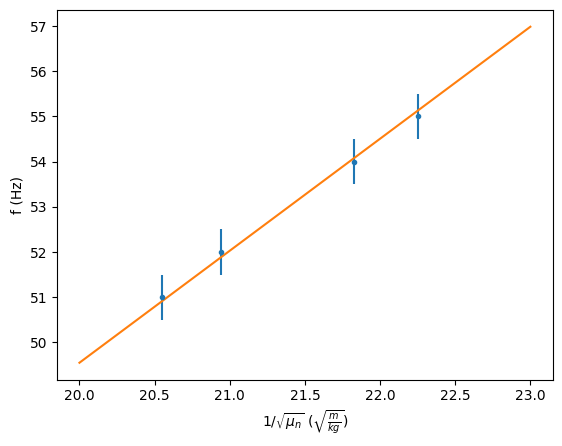
\includegraphics[width=0.6\textwidth]{Immagini/ML.png}
    \caption{Dipendenza della frequenza dalla radice quadrata della massa lineare di corde differenti.}
\end{figure}

Il test del $\chi^2$ evidenzia un ottimo accordo con il modello teorico: restituisce un $\Tilde{\chi}_o^2=0.06$, che per tre gradi di libertà restituisce una probabilità di accordo del 98.1\%.
Il coefficiente angolare interpolato è $k_{misurato} = \qty{2.48 \pm 0.01}{\hertz.kg^{\frac{1}{2}}.m^{-\frac{1}{2}}}$, mentre quello ricavato dalla relazione \eqref{eq:frequenze} è $k_{teorico} = \qty{2.38 \pm 0.05}{\hertz.kg^{\frac{1}{2}}.m^{-\frac{1}{2}}}$. Tramite la relazione \eqref{eq:t_test} si è ottenuto $t_0 = 1.88$, che corrisponde a una probabilità di accordo del 6.0\%: i valori risultano quindi marginalmente compatibili, ma è importante sottolineare che il coefficiente angolare misurato è comunque in accordo con quello teorico entro un intervallo di confidenza al 95\%.
